% declare documents and packages
\documentclass[man, 12pt, a4paper, nolmodern, noextraspace]{apa6}
\usepackage[T1]{fontenc}
\usepackage[utf8]{inputenc}
\usepackage[american]{babel}
\usepackage{csquotes}
\usepackage{amsmath}
\usepackage{amssymb}
\usepackage{microtype}
\usepackage{caption}
\usepackage{subcaption}
\usepackage{graphicx}
\usepackage{url}
\usepackage{times}
\usepackage{booktabs}
\usepackage{multirow} % multirow tables
\usepackage{arydshln} % dashline in tabular 
\usepackage{rotating} % vertical tables
\usepackage{pdflscape} % landscape pages
\renewcommand{\footnotesize}{\small} % use 11pt for footnotes
\usepackage[doublespacing]{setspace} % single space for footnotes
\setlength{\skip\footins}{1.5pc plus 1pt} % some more space between footnote and main body
% this command put all footnotes to endnote at the end of the paper
%\usepackage{endnotes}
%\let\footnote\endnote

% for word counts
\newcommand{\detailtexcount}{%
  \immediate\write18{texcount -merge -sum -incbib -dir \jobname.tex > \jobname.wcdetail }%
  \verbatiminput{\jobname.wcdetail}%
}
\newcommand{\quickwordcount}{%
  \immediate\write18{texcount -1 -sum -merge \jobname.tex > \jobname-words.sum }%
  \input{\jobname-words.sum} words%
}
\newcommand{\quickcharcount}{%
  \immediate\write18{texcount -1 -sum -merge -char \jobname.tex > \jobname-chars.sum }%
  \input{\jobname-chars.sum} characters (not including spaces)%
}

% Biblatex
\usepackage[style=apa,sortcites=true,sorting=nyt,backend=biber,uniquename=false]{biblatex}
\AtEveryBibitem{%
  \clearfield{issn} % Remove issn
  \clearfield{doi} % Remove doi
  }
% make in-text citations clickable
\usepackage[colorlinks=true]{hyperref}
% this removes annoying colors for in-text citation entries 
\usepackage{xcolor}
\hypersetup{  
    colorlinks,
    linkcolor={red!50!black},
    citecolor={blue!50!black},
    urlcolor={blue!80!black}
}

\addbibresource{CCR_lit.bib}
\DeclareLanguageMapping{american}{american-apa}
 
\title{When Does Garbage Start to Stink? Imperfect Gold Standards and the Validation of Automated Content Analysis}

\shorttitle{When Does Garbage Stink?}


\author{\addvspace{.25in} Hyunjin Song, Petro Tolochko, Jakob-Moritz Eberl, Olga Eisele, Esther Greussing, \\
        Tobias Heidenreich, Fabienne Lind, Sebastian Galyga, and Hajo G. Boomgaarden}

\affiliation{Department of Communication, University of Vienna, Austria}

\abstract{\centering TBA}

\keywords{Automated text analysis, reliability, validation, Monte-Carlo simulations}

\authornote{Please direct any questions and inquiries concerning this manuscript to \href{mailto:hyunjin.song@univie.ac.at}{hyunjin.song@univie.ac.at}}

\note{\addvspace{.25in} 
Draft date: \today \\
\addvspace{1in} 
Paper prepared for Inaugural issue of Computational Communication Research  \\
\addvspace{.25in} 
      \textbf{Draft in progress. Please do not cite without permission.} \\
      }

\begin{document}
    
\setcounter{page}{0}
\maketitle

    Automated text analysis methods become increasingly popular for analyzing texts in the social sciences, ranging from large-scale analyses of decades of newspaper coverage and party manifestos to millions of social media posts. Taking advantage of the fact that ever-growing quantities of text are available and have to be analyzed with limited resources, research in the social sciences nowadays readily turns to automated approaches to investigate a great range of questions in manifold sources \parencite{Boumans_Trilling_2016, grimmer2013text}. However, with the growing popularity of such approaches, the issue of the validity of obtained results and the conclusions drawn from them becomes crucial. Blindly applying automated approaches, and hence feeding algorithms or dictionaries into the machine without proper validation, may result in misleading or even plainly wrong findings; a principle famously illustrated by the phrase \enquote{garbage in, garbage out.}
    
    In this regard, such \enquote{text-as-data} approaches squarely depend on a proper validation of applied techniques against some gold-standard \parencite{grimmer2013text}.\footnote{Here, we use the term \enquote{gold-standard} and \enquote{ground truth} largely interchangeably, denoting some forms of objective data that serve as the reference.} Typically, applications of validation procedures using gold-standards rely on some human inputs (\enquote{human coding}) as a  benchmark to systematically compare and evaluate against proposed supervised methods-based or dictionary-based classifications. The most common practice here is to rely on precision (share of relevant items in all selected items), recall (share of selected items in all relevant items), and the resulting F1 score (ratio of precision and recall) of the automated procedure, using human coded material as a benchmark. Acting under the assumption that humans’ understanding of text outperforms that of machines and that, if trained correctly, humans will make mostly correct and valid classifications of texts, human coded data is treated as a gold standard against which the performance of the computer is judged. Consequently, the validation of computer-assisted coding based on human coded gold standards is grounded in the assumption that human readers’ placements or evaluations of a given text are indeed as close as we can get to an error-free, faultless and faithful representation of the quantities being estimated. However, “the quantities we seek to estimate from text [\ldots] are fundamentally unobservable” \parencite[p. 299]{lowe2013validating}, and human judgment is, in fact, no exception to this general rule -- as we know from the methodological content analysis literature. The consequences of, for example, human biases, predispositions and situational disturbances resulting in differing levels of “reliability” in human judgment in evaluating texts are well documented in traditional content-analytic applications \parencite[e.g.,][]{krippendorff2004reliability, hayes2007answering, lombard2002content, ennser2018impact}. Hence, the gold standard might not be as shiny as oftentimes assumed. By conditioning the relative performances of a given automated method against human inputs, we argue, the imperfect human coding (imperfect “gold standard”) greatly percolates a potentially already imperfect estimation of the automated procedures. Yet, the implications of using such imperfect human judgments as the benchmark for evaluating the validity of the results of automated text analysis – and especially the consequences of different levels of reliability in the gold standard are, until today, still insufficiently addressed.
    
    Against this backdrop, we first posit that a systematic validation of automated text analysis approaches is still rare in the social science literature, in general, and in communication research, in particular. Substantiating this argument, this study first presents a systematic review of articles published in the top social science journals in the past 20 years, showing that standards of validation are far from being acknowledged in the literature and that the reporting and interpretation of validation procedures differ greatly. More importantly, in a second step, we argue that by conditioning the performances of an automated method against human inputs, such validation procedures essentially mirror imperfect human performances. Therefore, using imperfect human judgments as the benchmark for automated text analysis validation effectively \enquote{tolerates} any mistakes or classification errors of automated procedures to a degree comparable to imperfect human judgments at researcher’s chosen degree of reliability levels. Thus, the choice of using human coding – and in particular the \enquote{quality} of such benchmarks – as a ground truth or gold standard may have systematic consequences for the evaluation of the proposed automatic procedures. 

    For this second step, we assess this previously unexplored connection between the quality of human judgment and relative performance of automated procedures (against true standards) by relying on large-scale, systematic Monte-Carlo simulations. Specifically, we illustrate how different levels of intercoder reliability scores in benchmark materials affect the assessment of overall (machine) accuracy/recall combinations (against such imperfect standards) and the ultimate conclusions drawn from such results. To our knowledge, our contribution is among the very first to provide a thorough, systematic evidence pertaining to a well-known, yet extremely scarcely discussed topic in automated content analysis. Our contribution should be read as a call for a systematic application of validation procedures in any social science publication drawing on automated text analysis procedures. At the same time, the study serves to benchmark the combination of reliability in gold standard/ground truth and validity scores and warns against improper use of both to demonstrate the validity of the approach. 
    
\section{Logics and Procedures of Automated Content Analysis}

    We define \enquote{automated content analysis} (or automated text analysis) as the collection of content-analytic approaches that utilize automated methods of coding a large amount of unstructured textual data, in a way that the coding process itself (i.e., the text classification) is not performed manually but rather done by predefined computational algorithms \parencite{trilling2018scaling, grimmer2013text}. 
    While the usage of the term \enquote{automated content analysis} in general in the extant literature encompasses a wide variety of forms \parencites[e.g., see:][]{riff2014analyzing, Hopkins_King2010, Krippendorff2013, grimmer2013text}, here we mainly supervised machine learning methods and a simple dictionary approach, wherein computational algorithms require a nontrivial degree of human decisions and inputs before or during the coding process itself \parencite{trilling2018scaling}. We choose to do so based on the consideration that many of the automatic content analysis applications in social science in general and in communication science in particular still heavily rely on those two broad approaches, although it is not uncommon to find the use of more sophisticated, yet highly flexible applications that have a slightly different focus \parencites[such as LDA topic models:][]{maier2018applying, dimaggio2013exploiting}. This study does not include unsupervised methods, since our primary interest is the interplay of human input and machine output. Also, our definition (inevitably) exclude automatic approaches of \textit{acquiring} textual data, or (more traditional) manual content analysis but merely make use of computers in tasks other than the actual coding process \parencites[such as in data entry or data management: e.g.,][]{lewis2013content}, although such aspects are, in practice, tightly intertwined with automated methods as we define here. 
    
    The prevalence of simple dictionary- or supervised learning-based methods is partly at least due to the fact that such forms of automated analyses are tend to be \enquote{designed to automate the hand coding of documents\ldots[in a way that] it will directly replicate the hand coding} \parencites[][p. 13]{grimmer2013text}. At the presence of a large volume of data, this can be an attractive option for overcomming the inherent time and resources constraints in manual approaches. In addition, in practice, such methods are relatively easy to implement in combination with manual approaches, which are still the dominant workhorse for many communication scholars.
    
    Although a specific method and application of automatic content analysis comes in many flavors \parencites[for a broad overview, see:][]{Boumans_Trilling_2016, grimmer2013text}, they are all based on similar principles: they all aim to identify and classify the predefined categories (i.e., a discovery and measurement).\footnote{In this respect, unsupervised learning methods are most clearly distinguishable from the other two: while unsupervised learning methods generally aim to inductively \enquote{discover} categories without human inputs, dictionary-based or supervised learning methods assume (already) well-defined categories. For a detailed discussion about the differences across methods, see \citeauthor{grimmer2013text} (\citeyear{grimmer2013text}) or \citeauthor{Boumans_Trilling_2016} (\citeyear{Boumans_Trilling_2016}).} A simple dictionary approach generally relies on the pre-defined “dictionary” of words or phrases by a researcher -- ranging from simple keywords lists to complex Boolean expression, syntactic parsers, or even regular expressions -- where the computer counts the number of such instances in a given document. Assuming a given dictionary is appropriate to be applied in a given domain \parencite{Boumans_Trilling_2016, gonzalez2015signals}, a researcher applies the dictionary on a set of documents, typically to a word-level, and then resulting \enquote{scores} are aggregated into the document level (e.g., a news article or tweet). This \enquote{dictionary} therefore represents a explicit coding rule to be applied by an algorithm, where (classified) categories may represent the visibility of a topic (i.e., the presence of the absence of a category) or a net tonality (positive vs. negative) of an article \parencites[e.g.,][]{Aaldering2016, YoungSoroka2012, boomgaaden2009, gonzalez2015signals, Rooduijn2011}. 
    
    For supervised methods, specific coding rules in manual annotations (as an input to an algorithm) are, in general, rarely explicitly articulated. Yet the algorithm takes such implicit judgments derived from manual coding as the point of reference, and tries to infer the features of data that best classify the text into different predefined categories. Currently, there exists a variety of supervised learning algorithms available -- ranging from a simple regression framework or Naive Bayes to more sofisticated methods such as Support Vector Machines (SVM) or random decision forest \parencites[for an overview of different algorithms commonly used in social science applications, see][]{hindman2015building}. This machine-learning process may involve many iterations of \enquote{training} and comparisons to some gold-standard materials in order to achieve a desired level of a classification quality \parencites[e.g.,][]{scharkow2013thematic}. If the algorithmic coding is later determined to be sufficient enough in capturing the underlying quantities of interest through such a \enquote{training,} then a researcher applies such \enquote{trained} coding rules to a larger corpus of unseen documents to perform their analyses \parencites[e.g.,][]{burscher2015using, burscher2014teaching, scharkow2013thematic, gonzalez2015signals}.    
    
\section{The Use of Human Coding in Cross-Validation of Automated Content Analysis}
    
    Just as the term \enquote{automated content analysis} itself, the notion of \enquote{cross-validation} often signifies many different practices within social sciences, although most of them usually involve some notions of triangulation. According to \citeauthor{Neunhoeffer2018} (\citeyear{Neunhoeffer2018}), there are at least four different meanings of cross-validation: (a) validating new measures or instruments (i.e., traditional measurement validity), (b) obtaining an \enquote{estimate} of \textit{true} error, (c) a model tuning (i.e., hyperparameter tuning), and (d) a robustness check using \textit{K}-fold validations (as a statistical tool). Yet for automated content analysis methods in particular, the discussion of \enquote{validation} has traditionally evolved around the first meaning of the term, following the general logic of establishing a correlative or a convergent validity of a measurement \parencites[][]{Krippendorff2008validity}. This is because any automated content analysis application -- at least the ones we are focusing on in this contribution -- essentially can be regarded as a classification problem (i.e., a measurement of the predefined categories in data). 
    
    In this respect, the most straightforward method of validating a measurement instrument (or rather the results thereof) is to compare one measurement with another measurement of the same concept. Therefore, applications of validation procedures in automated content analysis have traditionally relied on some sort of human inputs (“human coding”) as a benchmark, as discussed above. Since simple dictionary-based or supervised method-based automated coding essentially aims to produce human-equivalent judgment, there are indeed many steps within which a researcher can compare the manual coding of well-trained human coders and that of automated algorithms during a research process.
    
    In dictionary-based approaches, a great deal of labor-intensive human inputs are required when building and constructing a well-defined dictionary \parencite{YoungSoroka2012, muddiman2018re}.\footnote{Due to its labor-intensive nature of building a valid and reliable dictionary, recent applications in this topic are increasingly turn to \enquote{crowdcoding}, where the manual labor of highly trained yet few number of human coders are replaced with a large number of (untrained) crowd-coding workers \parencites[e.g.,][]{haselmayer2017sentiment, lind2017content}, serving as a \enquote{wisdom-of-the-crowd} approach. While a detailed discussion of such issue is beyond the scope of this article, interested readers may instead consult \citeauthor{lind2017content} (\citeyear{lind2017content}).} Yet once created, the actual coding process itself using the dictionary does not involve any human inputs. Instead, the use of manual coding in dictionary approaches may involve additional comparisons of the derived results against manual coding, in a sense that such comparisons are often made \textit{post-hoc} for validating the results. \citeauthor{Rooduijn2011}'s (\citeyear{Rooduijn2011}) research on the (automatic) measurement of \enquote{populism} in election manifestos well exemplifies the use of human coded data in validating the results of automated approaches. Using a traditional manual content analysis, they show dictionary-based automatic coding of \enquote{populism} categories in party manifestos produces essentially very similar results compared to manual coding. Similarly, \citeauthor{YoungSoroka2012} (\citeyear{YoungSoroka2012}) compare the manually coded newspaper content against the results based on Lexicoder Sentiment Dictionary (LSD), and found that results using LSD and manual content analysis are largely comparable to each other.
    
    Nevertheless, most often such dictionaries are validated during the initial dictionary construction processes, and it is exceptionally rare to see a validation of results \textit{after} such classification tasks \parencites[yet for notable exceptions, see][]{muddiman2018re, YoungSoroka2012, gonzalez2015signals}. Once the dictionary is created and tested, one typically assumes the classification membership that has to be estimated by an algorithm to be a simple additive --- and only exclusive --- function of the given dictionary elements (i.e., aggregation of positive and negative dictionary scores results in the general sentiment of the article, etc.), typically ignoring any residual textual features that are not captured by a given dictionary features. Such blind trust in the dictionary grossly misses the very likely possibility that a given text in question (i.e., a newspaper article or a social network post) is more than a simple sum of its parts. Admittedly, the researchers frequently make such an assumption the minute before they decided to use a dictionary, however to our knowledge little to no validation has been done in substantive studies that utilizing dictionaries for classification purposes to check how well does a given dictionary approximate the objective reality of text data.
    
    In supervised methods, the role of human input is more central in fine-tuning the algorithm (i.e., an \enquote{inner} cross-validation). As exemplified in \citeauthor{scharkow2013thematic} (\citeyear{scharkow2013thematic}), in supervised methods a researcher typically produces manually annotated sample materials, or \enquote{training set,} and the algorithmic classifier is later trained on sample material in order to develop certain statistical models (that effectively aim to reproduce implicit coding rules of human coders) to predict and classify unseen materials, the \enquote{test set.} As such, human inputs are more directly utilized in such \enquote{learning} procedures in supervised methods, as opposed to being utilized post-hoc as in dictionary approaches. For instance, \citeauthor{burscher2014teaching} (\citeyear{burscher2014teaching}) have developed a supervised machine-learning algorithm to automatically classify certain generic media frames in news articles, based on random subset of data that were manually coded by trained coders.\footnote{In unsupervised methods, the use of human-coding as a benchmark is a common practice as well. For instance, \citeauthor{lowe2013validating} (\citeyear{lowe2013validating}) directly compare direct human-coding based party position scaling (which serves as a benchmark) against unsupervised scaling methods, found that the proposed parametric scaling methods can produce largely similar results on par with human judgments.} Yet due to inherent resource constraints associated with human coding, such validations typically rely on only a small subset of held-out samples to provide annotations that establish the ground-truth. As such, although in principle a researcher can further validate their final outcomes by relying on an additional post-hoc validation method as described in dictionary-based approaches (i.e., an \enquote{outer} validation), this is rarely offered in practice.   
    
\section{The Myth of Perfect Standard in Human Coding?}

    Regardless of its specific orientations briefly reviewed above, in extant literature \enquote{human reasoning is routinely described as a 'gold standard' against which algorithmic output should be judged} \parencites[][p. 2]{dimaggio2015adapting}. Indeed, the use of human coding as a gold standard is often regarded as \textit{the} principal method of ensuring the validity and soundness of conclusions derived from the proposed automated procedures \parencites[e.g., ][]{grimmer2013text, lowe2013validating}. The purpose of such cross-validation against a gold standard is, as \citeauthor{Krippendorff2008validity} (\citeyear{Krippendorff2008validity}) notes, \enquote{to confer validity on the otherwise uncertain research results} (p. 6). Admittedly, this logic requires that the chosen benchmark (i.e., manually produced annotations by human coders) to be of \enquote{objective} and \enquote{unquestionable} truth --- which, we anecdotally observe, is more common among natural language processing and sentiment analysis literature \parencites[e.g.,][]{dimaggio2015adapting}. Yet as much of the traditional manual content-analytic literature suggests \parencites[][]{krippendorff2004reliability, hayes2007answering, lombard2002content, ennser2018impact}, manual coding more often than not easily produces unreliable judgments as well, and especially more so when the judgment in hand requires a nontrivial degree of inferences and subjectivity to classify a latent information in a given text \parencites[][]{riff2014analyzing, Krippendorff2013}.       
    
    The issue of (inter-coder) reliability is one of the most essential concerns in the extant literature concerning the quality of manual content analysis. If the reliability estimates of key constructs are not that compelling, as \citeauthor{Krippendorff2013} (\citeyear{Krippendorff2013}) notes, \enquote{doubts as to what these data mean prevail, and their analysis is hard to justify} (p. 268). As such, there has been relatively little disagreement regarding the consequences of sub-optimal reliability for key measurements \parencites[][]{krippendorff2004reliability, Krippendorff2013}, and the need for better reliability for that matter, at least for many recent manual content analysis applications. Yet to date, little attention has been devoted to the question of how the \enquote{quality} of manual coding affects the validity and conclusions derived from automated procedures. This is especially surprising, since -- as \citeauthor{dimaggio2015adapting} (\citeyear{dimaggio2015adapting}) notes -- \enquote{whenever ... principles by which humans generate ratings are heterogeneous across raters} (p. 4), any automated procedures that are systematically evaluated upon such imperfect human input will be biased to the degree that can be found in such biased human judgments. 
    
    The use of (potentially) imperfect human coding as an ultimate benchmark against which automatic techniques are validated upon may have therefore at least two systematic consequences. First, while automated methods themselves are perfectly reliable in producing the same results whenever repeated, imperfect human judgments (on validation materials) essentially makes the ultimate \enquote{target} of such perfectly reliable measurements radically deviate from the \enquote{true} target of inference, making them \enquote{reliably wrong} on-target. Second, and somewhat relatedly, systematically flawed human judgment can bias the performance of learning algorithms, leading to biased conclusions against a true standard. Therefore, using imperfect human coded data as an ultimate benchmark makes it harder to evaluate the relative trustworthiness of such validation procedures. However, most of the studies do not provide any validation at all (please see our later empirical section), or even among studies which \textit{do} compare automated procedures with manual coding as a validation tool, they often misreport or misspecify the validation metrics and hardly ever report the quality of such manual coding itself but essentially treat such imperfect human judgment as \textit{the} true, gold-standard materials \parencites[e.g.,][]{gonzalez2015signals, lowe2013validating, YoungSoroka2012}. Indeed, we know only one existing study \parencite{burscher2014teaching}, which suggests some tentative evidence between quality of human coding and (machine-based) classification accuracy.\footnote{In a recent study, \citeauthor{gonzalez2015signals} (\citeyear{gonzalez2015signals}) compare five available sentiment dictionaries against human annotations, yet they do not directly deal with the implications of imperfect reliability in human coding. \citeauthor{scharkow2017measurement} (\citeyear{scharkow2017measurement}), the only one of existing studies that examines the consequences of imperfect reliability in human coding, mainly deal with its implication on \enquote{linkage analysis}, but not on automated content analysis.}     
   
    In sum, there appears to be a convincing reason to suspect a systematic relationship between the quality of human coding and the relative bias and errors regarding the ultimate conclusions from the automated content analysis -- especially when using such imperfect human coding as the ``gold-standard''. While many of prior contributions on this topic -- both theoretically and empirically -- stresses a need for a proper validation of applied techniques against some gold-standard \parencites[e.g.,][]{grimmer2013text, Hopkins_King2010, gonzalez2015signals}, we do not know much about how the field in general stands in terms of standard validation practices and the use of imperfect human coding in particular. Therefore, we first conduct a systematic review of relevant articles published in the top social science journals in the past 20 years, focusing on the use of manual coding (by trained human coders), if any, in standard validation procedures against the proposed automated methods, and the assessment of performances of such automated methods (Study 1). While this systematic review should provide us a overall picture of typical validation procedures in any publication drawing on automated text analysis procedures in extant literature, study 1 at the same time further serves to benchmark in modeling the combination of reliability in gold standard/ground truth and validity scores against the true standard (Study 2), where we warn against improper use of both to demonstrate the validity of the approach.

\section{Study 1: A Content Analysis Study}

\subsection{Sample and Procedures}

    We have identified relevant studies using the EBSCO host databases “Communication \& Mass Media Complete,” “Humanities Source,” and “SocINDEX with Full Index,” querying all abstracts and corresponding keywords using the following Boolean search string: “("computer-assisted" OR "computer assisted" OR "automated" OR "automatic" OR "computational" OR "machine learning") AND ("content analysis" OR "text analysis").” This resulted a total of 192 relevant papers. Among them, \textcolor{red}{95} articles were determined not relevant (e.g., an overview/introduction article, qualitative analysis, or studies using unsupervised methods or simple keyword frequencies, etc), therefore excluded from the further analysis. Using remaining 97 articles, we systemically examined whether extant applied studies using dictionary- or supervised methods a) adequately employ any cross-validation of their primary findings, b) if so, whether they use human coded materials as a benchmark, and c) if so, whether intercoder relabilities and other methodological details are adequately and consistently reported. 
    
    A total of five highly qualified coders tested the initial coding scheme developed by the first and third author by independently coding 10 sample articles (approximately 10\% of total sample) and collectively discuss the coding problems and disagreement. Based on this iterative procedure, coding instructions were revised until the coding schemes would produce reliable results among any trained and competent coders. Intercoder reliability was assessed for each of the variables coded, using Krippendorff’s alpha, which is reported in Table XX below.   
    
\subsection{Results}

    The results for each variables examined are presented in Table XX below. 

\section{Study 2: A Monte-Carlo Simulation Study}
    
    The result of Study 1 reveals \textcolor{red}{TBA}. 
    
    In order to systematically evaluate how different setups and practices of utilizing manual coding within automated procedures can yield different conclusions, we setup an extensive set of Monte Carlo (MC) simulations (\textit{N} = 240,000). MC simulation offers a convenient tool for systematically evaluating the relative bias and coverage of a given statistic under certain scenarios \parencites[for an example, see][]{scharkow2017measurement, leemann2017extending}. 
    
    While we setup our procedures in a way that largely mirrors the typical approaches in this area, dictionary approaches and supervised learning approaches considerably differ in how they utilize manual coding, as well as their data requirements and the logic underlying each of the technique. Therefore, here we develop two separate approaches in simulating their behaviors. Yet in all of the cases, we have broken down our approach into three stages – data generation, human coding, and automatic classification – where we systematically vary the intercoder reliability of the “gold standard” material, along with a number of related factors such as number of coders and the number of manual annotations per coder (see below section). Then we systematically compare different scenarios in terms of their precision, recall, and F1 scores based on the \enquote{true} standard (i.e., a quantity of interest that is typically unknown to researchers) in order to illustrate how different practices of human coding in automated content analyses affect the overall results and the relative trustworthiness of conclusion drawn from such results.
    
    \subsection{Data Generation Stage}
    
    We create data (e.g., textual data to be analyzed by a researcher) with the \enquote{true} outcome variable of interest; the goal of any quantitative text analysis method is somehow approximate the true value \textit{y}, either by human coding, machine algorithms, or some combinations of both. For the data generating process, we set the true value of \textit{y} to be stochastically generated from three hypothetical independent variables ($x_1$, $x_2$, and $x_3$), the values of which were sampled either from a multivariate normal distribution (for supervised learning) or from a categorical distribution (for dictionary approach -- see below). We assume the size of text data is sufficiently large to warrant an automated approach. As such, the data in question (hypothetically) covers 10 news articles per day per each of 10 media outlets, spanning a total of 20 years. Accordingly, each single simulation run is set to generate 730,000 observations (10 x 10 x 365 x 20).
    
    \subsubsection{Supervised ML Scenario}
    For supervised learning scenarios, we assume values of independent variables are sampled from a multivariate normal distribution, with a randomly generated variance-covariance matrix \textbf{$\sum$} for each simulation run. This randomly generated variance-covariance matrix ensures that idiosyncratic values of the covariance matrix do not skew the overall results of the simulation. The \textit{true}  values of $y$ (which is the binary variable) are then sampled from a Binomial distribution, with the probability parameter having a very simple linear functional form as follow:
    \begin{equation}
        \begin{gathered}
            y \sim Bernoulli(\pi) \\
            \pi = logistic(\mu) \\
            \mu = \boldsymbol{X\beta} + \epsilon
        \end{gathered}
    \end{equation}
    \noindent with $\epsilon$ being Gaussian noise added to ensure that each run of the simulation is not completely deterministic. The $\boldsymbol{\beta}$, true population parameters, were fixed throughout the simulation runs (specifically, $\beta_1$ = .5, $\beta_2$ = .2, and $\beta_3$ = .6, which were randomly chosen). 
    
    \subsubsection{Bag-of-Words Scenario}
     For a dictionary (bag-of-words) method, we assume a very similar approach to data generation as discussed above, however we assume values of independent variables were sampled from a Categorical distribution with a separate Dirichlet priors for negative and positive draws (i.e., a discrete value range range from -5 to 5), where they represent some \enquote{features} of a given textual data (e.g., a word or N-grams). These values are later to be matched with a \enquote{dictionary} (which has similar discrete values that represent a predefined category) in order to determine the estimated values of $y$ for each observation. Since this requires discrete rather than continuous values, here we use slightly different setup for the dictionary approach:
       \begin{equation}
        \begin{gathered}
            \pi_{neg} \sim Dirichlet\bigl(N, \alpha_{neg}\bigr) \\
            \pi_{pos} \sim Dirichlet\bigl(N, \alpha_{pos}\bigr) \\
            \boldsymbol{X}_{k \in K}^T \sim Categorical\bigl(N, \bigl[\pi_{neg}\ \textrm{or}\ \pi_{pos}\bigr]\bigr) \\
        \end{gathered}
    \end{equation}
    \noindent with $N$ being the total number of observations, and $\alpha_{neg}$ and $\alpha_{pos}$ --- concentration hyperparameters with mass concentrated closer and further away from 0, respectively, $\boldsymbol{X}_k$ being a single independent variable, and $K$ being the desired number of variables. The two negative and positive Dirichlet priors $\pi_{neg}$ and $\pi_{pos}$ are randomly selected for each draw when a single column of independent variables is drawn, treating such independent variables as a systematic, recurring features of a given textual data. Having generated the set of independent variables of textual features, we generate $y$ in a similar fashion as discussed in (1), such that the \textit{true} values of \textit{y} are then sampled from a Binomial distribution as discussed above. Yet for the bag-of-words approach, the vector $\boldsymbol{\beta}$ is extended to K = 5 and their $\boldsymbol{\beta}$ values are fixed to .2 in order to better approximate the dimensionality of text data and reflect the possibilities of potential feature misspecification. This means that $y$ becomes effectively a function of the simple sum of chosen textual features. 

    \subsection{Human Coding Stage}
    
    We specified several typical scenarios of how the true data would be coded by human coders for the purpose of validation of automated procedures. In typical automatic content analysis applications, at least two or more number of trained human coders are assigned to a common, small set of sample documents for manual coding, and independently code such documents for intercoder reliability testing. This process is repeated until the level of intercoder reliability is deemed satisfactory (typically Krippendorff’s alpha equal or greater than 0.7). Theoretically, achieving the satisfactory level of reliability means that coders can be treated as interchangeable to each other \parencite{krippendorff2004reliability}, therefore any observations produced by a single human coder in validation materials are, on average, likely to be similar to each other proportional to the chosen degree of intercoder reliability. Once such a coder interchangeability is ensured, the common practice is that remaining documents (for validation materials) are evenly --- typically by some convenient standard but non randomly --- divided and only coded by a single coder \parencite{grimmer2018unreliability}. While the total number of manual annotations produced by such human coders greatly vary across studies, the practice of evenly (but not randomly) dividing the validation materials across coders effectively means that any potential coder idiosyncrasies are just ignored while such idiosyncrasies are not randomly distributed across manual annotations produced for validation materials.      
    
    Following the typical application in this area as sketched above, we assume that only a small fraction of data (i.e., held-out sample) is analyzed manually by a varying number of human coders for the purpose of providing a cross-validation result (against machine algorithms) that informs the performance of such automated procedures. Following this general setup \parencites[e.g.,][]{grimmer2018unreliability}, we specified few important factors that may affect the quality of the “golden standard” and therefore of the overall performance evaluation of later automated content algorithms. Those factors include: the number of human coders (k = 2, 4, 7, 10), the predetermined target values of intercoder reliability metric (Krippendorff's alpha = 0.5, 0.6, 0.7, 0.8, 0.9), as well as the number of articles that each coder had to analyze in order to produce final human-coded data (the number of annotation per coder, n = 50, 100, 250, 500). Although somewhat arbitrary, these numbers were chosen to reflect typical content analysis procedures and their variations commonly carried out in social science applications, as evidenced in our Study 1. 
    
    In all scenarios, human coders classify a given observation as ``1'' (e.g., a news article contains the quantity of interest, such as a certain actor, frame, or tonality) or ``0'' (e.g., does not contain this quantity of interest). This human coding ($\hat{y}$) can be in principle either correct or incorrect against the (unknown) “true” value of $y$, therefore behaviors of human coders were modeled by a Binomial distribution with varying probability of successfully categorizing the true data. The heterogeneity in each of the coders’ coding behaviors (e.g., expertise or bias) was also modelled by a beta distribution with varying shape (using predefined hyperparameters for each target reliability levels), which effectively enables us to simulate a situation in which where a certain coders produce more “correct” judgment ($\hat{y} = y$) whereas other coders produce more ``false'' judgment ($\hat{y} \neq y$). Yet the overall human annotation patterns at chosen level of a beta distribution parameters were ensured to produce an acceptable level of target reliability coefficient (e.g., Krippendorff's alpha = 0.7). Depending on specific application (dictionary-based vs. supervised learning), the output (coded data) from this stage is then used as either a post-hoc validation data or as an input for the later automated classification stage. 
    
    \subsection{Algorithm-based Classification Stage}
    
    Following the typical application, we assumed a researcher uses a certain classification algorithm to predict the values of ($\hat{y}$) in each of the observations. For this purpose, we used three different classification algorithms – binomial GLM, Naïve Bayes (NB) classifier, and a bag-of-words dictionary approach. Although these are not exhaustive, these methods are among the most frequently utilized applications in automated contents analysis, especially coupled with human validation of such algorithms, as can be seen in \textcolor{red}{Table 1 in our Study 1 result}. 
    
    Typically in a real-world scenario, researchers validate the computer-based coding based on a held-out human coded test set post hoc (for a bag-of-words dictionary approach), or use such human coded data to develop prediction algorithms and then ``scale up'' the automated coding process (for supervised learning, such as binomial GLM or Naïve Bayes). This means that we can also systematically compare different levels of precision, recall, and F1 scores (that are evaluated at different levels of human benchmark scores) against the true standard. For this purpose, we compare the estimated $\hat{y}$ values from scaled-up automated coding to the true values of y. Admittedly this would be impossible for practical applications, since the true value y would never be known. However by doing so, we can precisely estimate the relative bias when using imperfect human coding as \enquote{gold standard} while further can compare how the overall accuracy is diminished from one step to another based on which factors. 
    
    The final Monte Carlo simulation used 4 (number of human coders, k) $\times$ 5 (target Krippendorff's alpha levels in human coding) $\times$ 4 (N of annotation per each human coder in producing validation data) $\times$ 3 (classification algorithms) full factorial design with 1,000 replications per each scenario, therefore yielded 240,000 results, which then summarized below.
    
\section{Simulation Results}

As a model check, we first investigate the overall classification accuracy (against true value) as a function of target reliability level in validation materials, predicting how well the proposed algorithms correctly predict the quantity of interest (such as a certain actor, frame, or tonality) at varying level of reliability level in validation materials. In Figure \ref{fig:Figure1} below, different levels of target Krippendorff's alpha is stacked over y-axis in each panel, and in x-axis overall prediction accuracy against true value (defined as the proportion of correct predictions, or the sum of true positive and true negative cases over entire cases) are presented along with their 95\% confidence intervals, for every combination of experimental factors in MC simulations.

\centerline{ -- Figure \ref{fig:Figure1} about here -- }    
    
% Figure 1: Overall accuracy
\begin{figure}
         \captionsetup[figure]{labelfont=bf,textfont=normalfont,singlelinecheck=on}
         \centering
         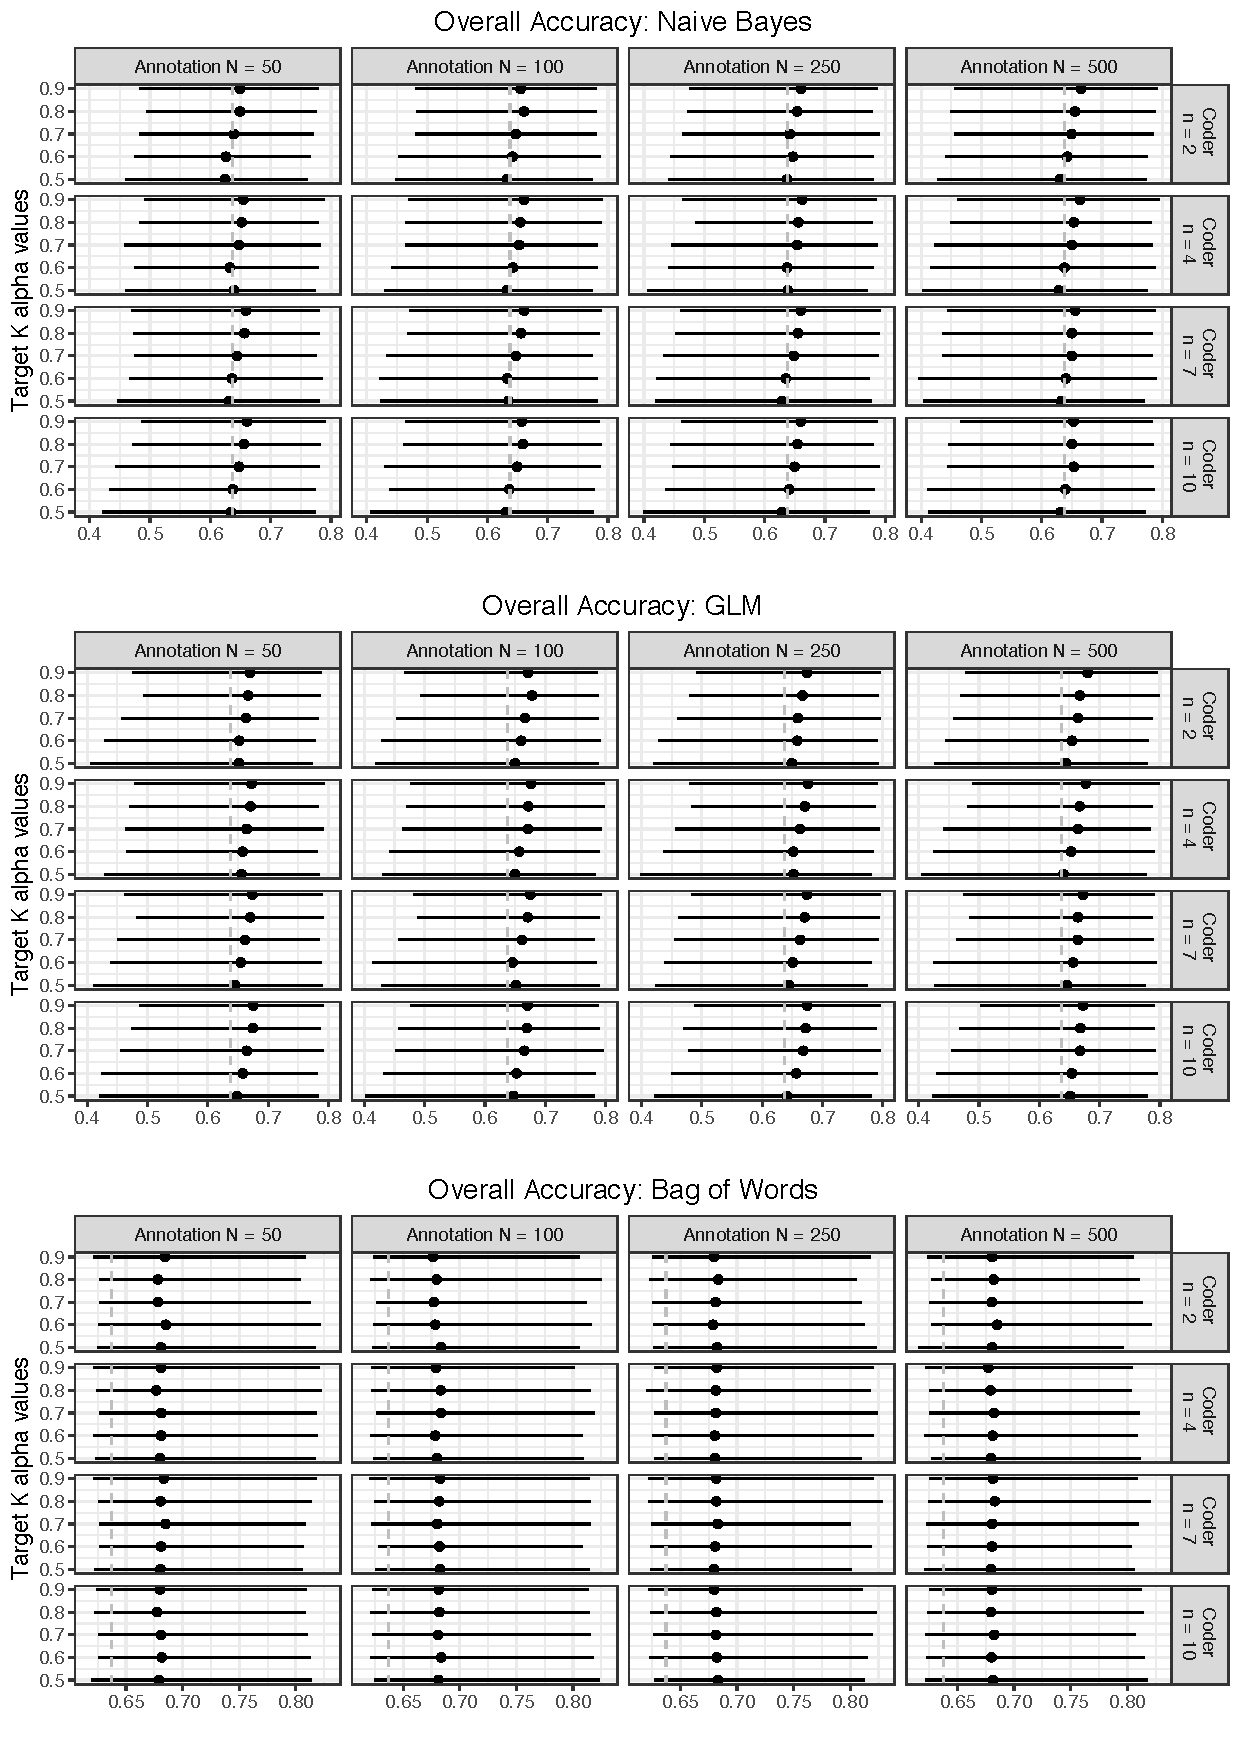
\includegraphics[trim={0.2cm 0.2cm 0.2cm 0.2cm}, clip, width=\columnwidth]{Results/overall_accuracy.pdf} 
         \captionsetup{format=hang}
         \caption{Overall classification accuracy against true value across conditions (Reference line is overall mean).} 
         \label{fig:Figure1}
\end{figure}    

As can be seen in Figure \ref{fig:Figure1} above, within two ML scenarios, using \enquote{better} quality training material appears to directly increase true classification accuracy, which is expected results. Using the overall accuracy in our simulation as the reference point, the first and the second panels of Figure \ref{fig:Figure1} makes it clear that the reliability level of training material have a nontrivial benefit in improving the accuracy of prediction based on automated procedures. Indeed, this is somewhat expected results since the ML methods takes the human input as the bases of developing classification algorithm, therefore overall accuracy of the final classifier is dependent upon human input and its quality thereof. In contrast, the last panel of Figure \ref{fig:Figure1} shows that typical Bag-of-words application does not benefit from improved (post-hoc) human coding. Yet again, this is much expected pattern, since in typical dictionary application, the quality of a given dictionary itself does not depend at all on post-hoc human coding unless such human coding is used in developing and constructing dictionary itself. Overall, our results presented in Figure \ref{fig:Figure1} shows that our simulation setup can correctly reproduce a common expected pattern in extant studies (therefore ensures the validity of our analysis and conclusion).   

Next, we examine indirect consequences of relying on imperfect human coded materials as a benchmark in evaluating the performances of automated procedures in terms of post-hoc validation. Typically, researchers rely on  small fraction of human-coded materials for validating their primary findings from automated procedures, deciding whether the overall accuracy or classification performance is good enough to proceed to further analyses, based against some \textit{a priori} chosen threshold value: if validation (based on human coding) is purportedly not satisfying enough to pass such a threshold level, additional steps are sought to improve the quality of automated procedures (e.g., re-training of algorithms, or changing the dictionary, etc).\footnote{Here, we do not consider a scenario where a researcher decides to improve the quality of human coding. This is based on the consideration, as to our argument being advanced here, that a researcher (often incorrectly) assumes that human coding is perfectly reliable and valid.} The primary interest of such post-hoc validation procedures lies in extrapolating the observed level of classification performance (based on validation materials) to the level of classification performance \textit{that could have been observed} based on entire range of data. In other words, the observed level of classification performance serves as a proxy, or an estimate for the true, unknown classification performance. Therefore, interesting question here is how well the observed classification performance reflects true classification performance under imperfect reliability, and how large or small a potential bias is. Relatedly, making decisions about the unknown, true values of overall classification performance based on observed performance from hand-coded validation materials, essentially, can be seen as classical decision error scenarios (i.e., type I and type II errors), as schematically presented in Table \ref{tab:Table1}.
\centerline{ -- Table \ref{tab:Table1} about here -- }    

% Table 1
\begin{table}[!htbp] \centering 
	\begin{minipage}{1.1\textwidth}
    \centering
  \caption{\\ Decision scenarios based on observed vs. true level of classification performance.} 
  \label{tab:Table1} 
        \centering
  \begin{tabular}{ ccc}
\toprule
      \multicolumn{1}{c}{} &
      \multicolumn{2}{c}{\textbf{True classification performance}} \\
\cline{2-3}
 & Below threshold & Above threshold \\
\hline \\[-1.8ex] 
  \textbf{Observed} & & \\  
 Below threshold & True Negative & False Negative (Type II) \\ 
 Above threshold & False Positive (Type I) & True Positive \\ 
\hline \\[-1.8ex]  
	\end{tabular}
 	\end{minipage}
\end{table} 

In order to illuminate the potential consequences of relying imperfect data in making decisions about the true, unknown classification performances of the proposed automated procedure, we divide our entire simulations into four mutually exclusive categories, as in Table \ref{tab:Table1}, based on the cross-tabulation of \enquote{observed} F1 scores (from validation materials) against true F1 scores (based on the true values of y). We first present the proportion of simulation cases which incorrectly conclude about the overall classification quality based on observed quality. Second, we further present the degree of relative \enquote{bias} within such incorrectly concluded cases --- defined as the $ F1_{validation}/F1_{true} $, where F1 score is a weighted average of the precision and recall --- which captures the degree of under- or over-estimation of (true) overall F1 scores against observed F1 scores based on human validation materials. For this application, we choose the cutoff value of F1 score to be 0.6478, which is just the average F1 score reported in Study 1.
\centerline{ -- Figure \ref{fig:Figure2} to Figure \ref{fig:Figure4} about here -- }    

% Figure 2 proportion of decision error, Naive Bayes
\begin{figure}
\captionsetup[figure]{labelfont={bf,it}}
    \centering
    \begin{subfigure}[t]{0.95\textwidth}
        \centering
        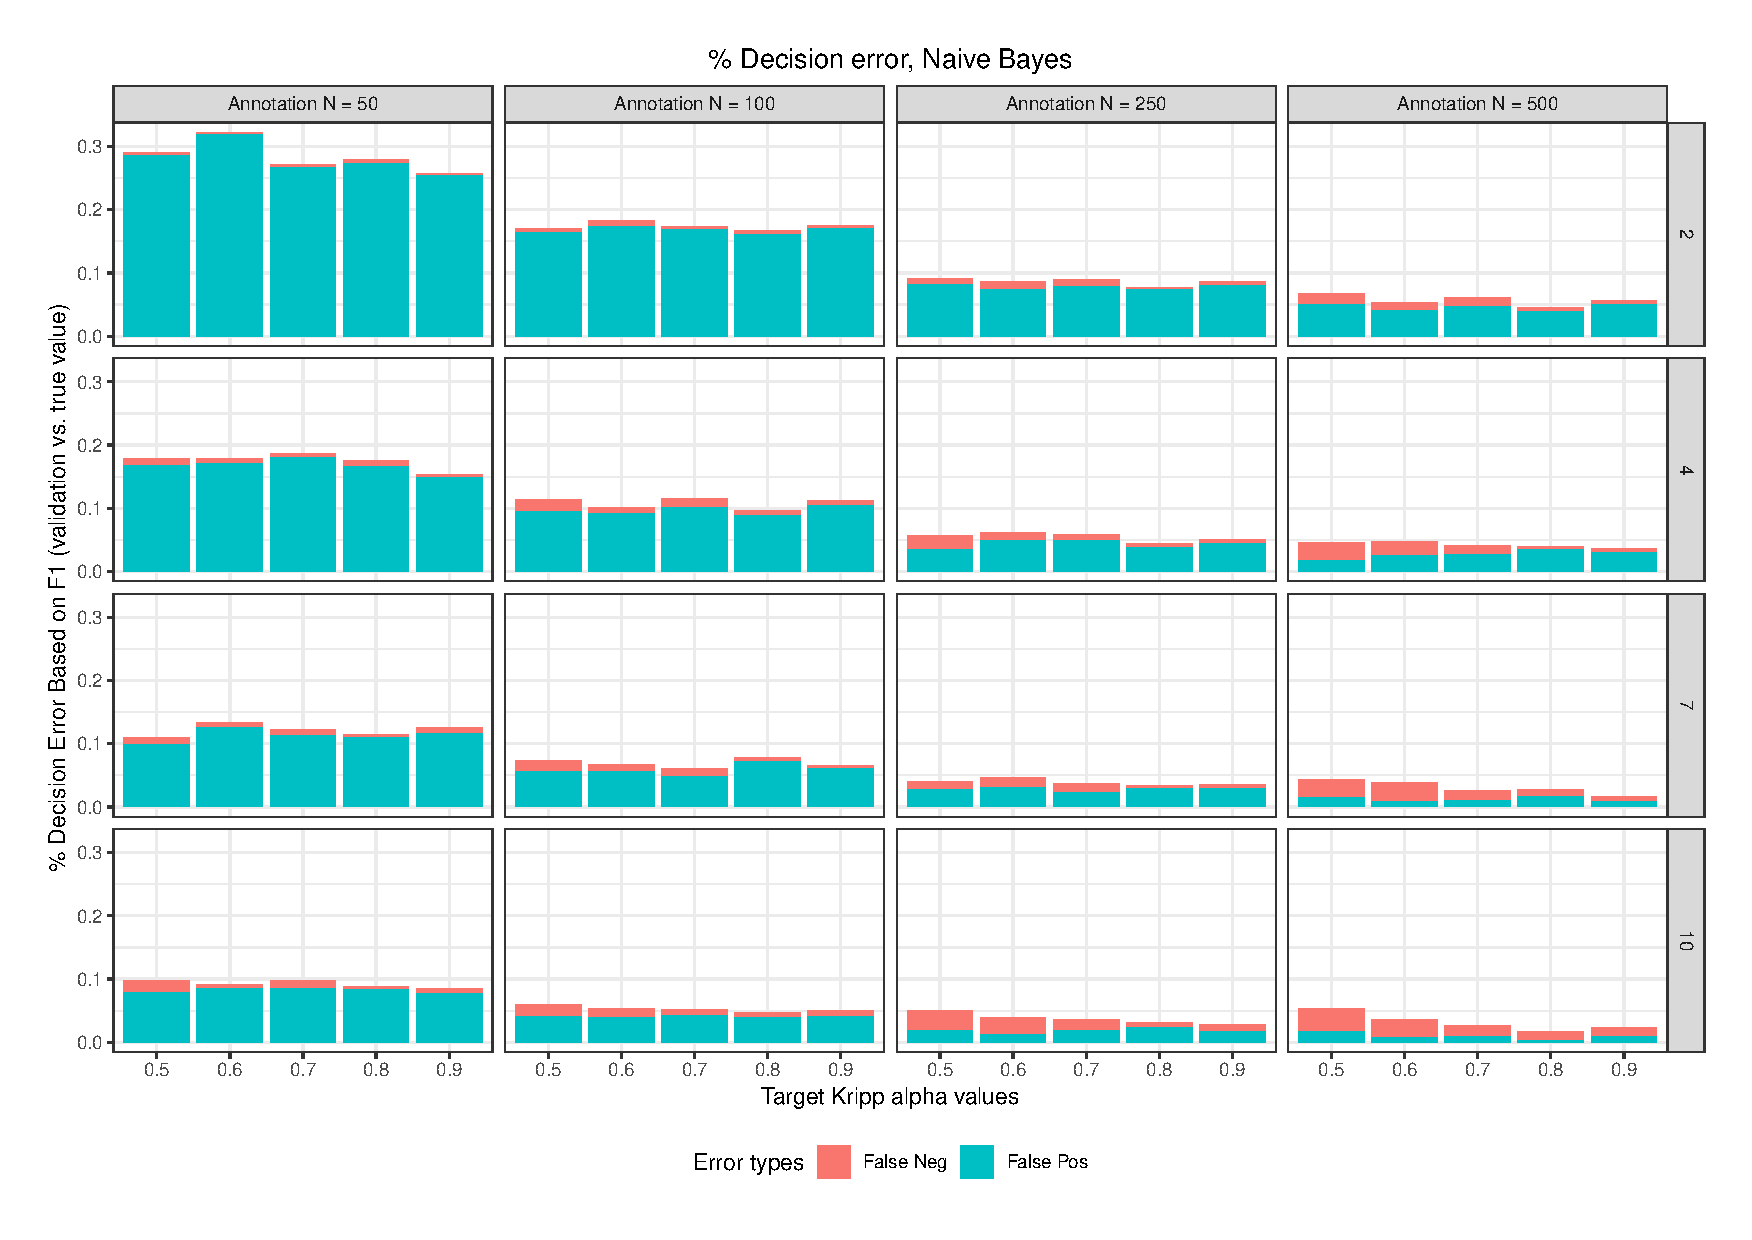
\includegraphics[clip, width=\linewidth, page = 1]{Results/BAYES_summary_05.pdf} 
    \end{subfigure}
    \begin{subfigure}[t]{0.95\textwidth}
        \centering
        \captionsetup{font=small}
        \includegraphics[clip, width=\linewidth, page = 2]{Results/BAYES_summary_05.pdf} 
    \end{subfigure}
    
    \captionsetup{format=hang}
    \caption{Percentage of decision error and relative bias in F1 scores (over 1000 Simulations per each scenario), Naive Bayes classifier.} 
    \label{fig:Figure2}
    \captionsetup{font=small}
    \caption*{Note: Upper panel = Proportion of cases (each simulation run) incorrectly conclude on classification performances. Lower panel = Relative bias in F1 scores among misclassified studies.}
\end{figure}          

% Figure 3 proportion of decision error, GLM
\begin{figure}
\captionsetup[figure]{labelfont={bf,it}}
    \centering
    \begin{subfigure}[t]{0.95\textwidth}
        \centering
        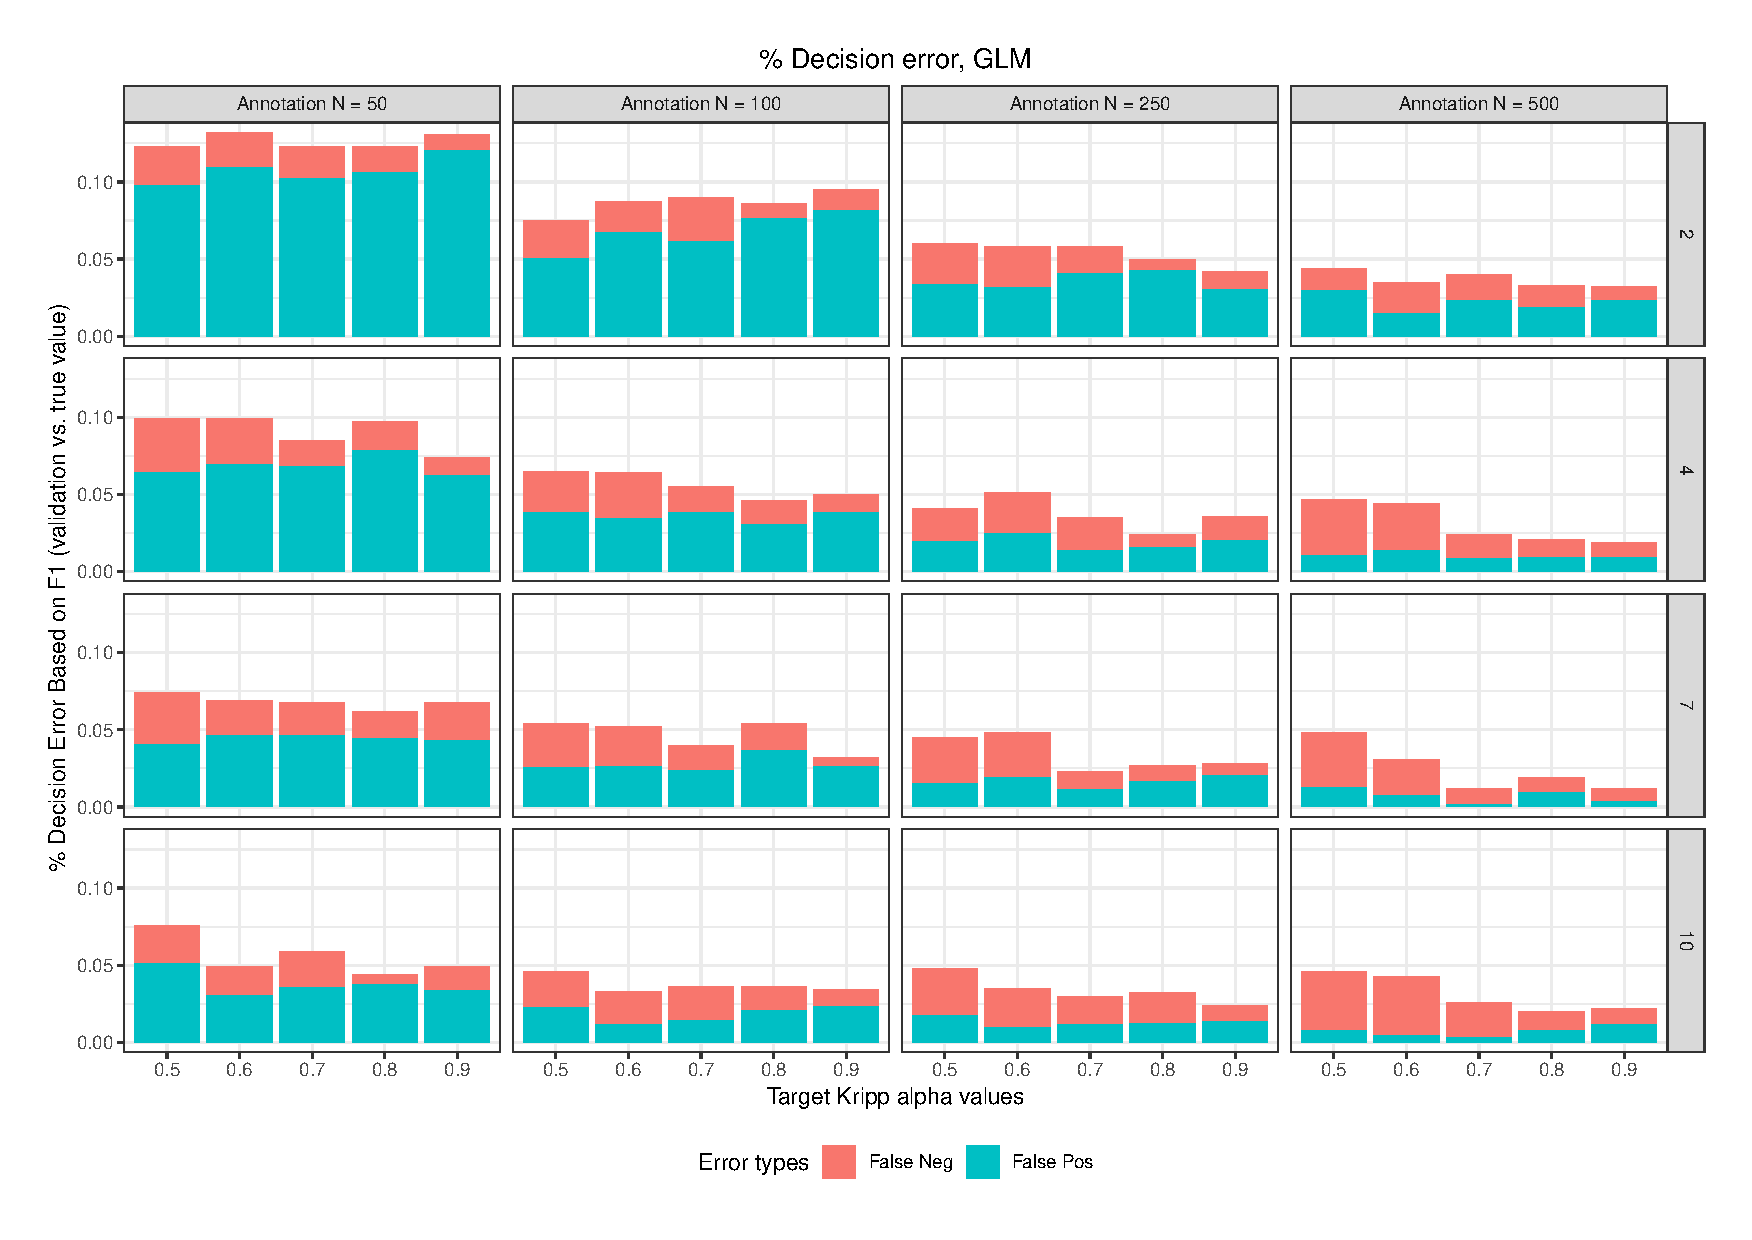
\includegraphics[clip, width=\linewidth, page = 1]{Results/GLM_summary_05.pdf} 
    \end{subfigure}
    \begin{subfigure}[t]{0.95\textwidth}
        \centering
        \includegraphics[clip, width=\linewidth, page = 2]{Results/GLM_summary_05.pdf} 
    \end{subfigure}
    
    \captionsetup{format=hang}
    \caption{Percentage of decision error and relative bias in F1 scores (over 1000 Simulations per each scenario), GLM classifier.} 
    \label{fig:Figure3}
    \captionsetup{font=small}
    \caption*{Note: Upper panel = Proportion of cases (each simulation run) incorrectly conclude on classification performances. Lower panel = Relative bias in F1 scores among misclassified studies.}
\end{figure}     

% Figure 4 proportion of decision error, BoW
\begin{figure}
\captionsetup[figure]{labelfont={bf,it}}
    \centering
    \begin{subfigure}[t]{0.95\textwidth}
        \centering
        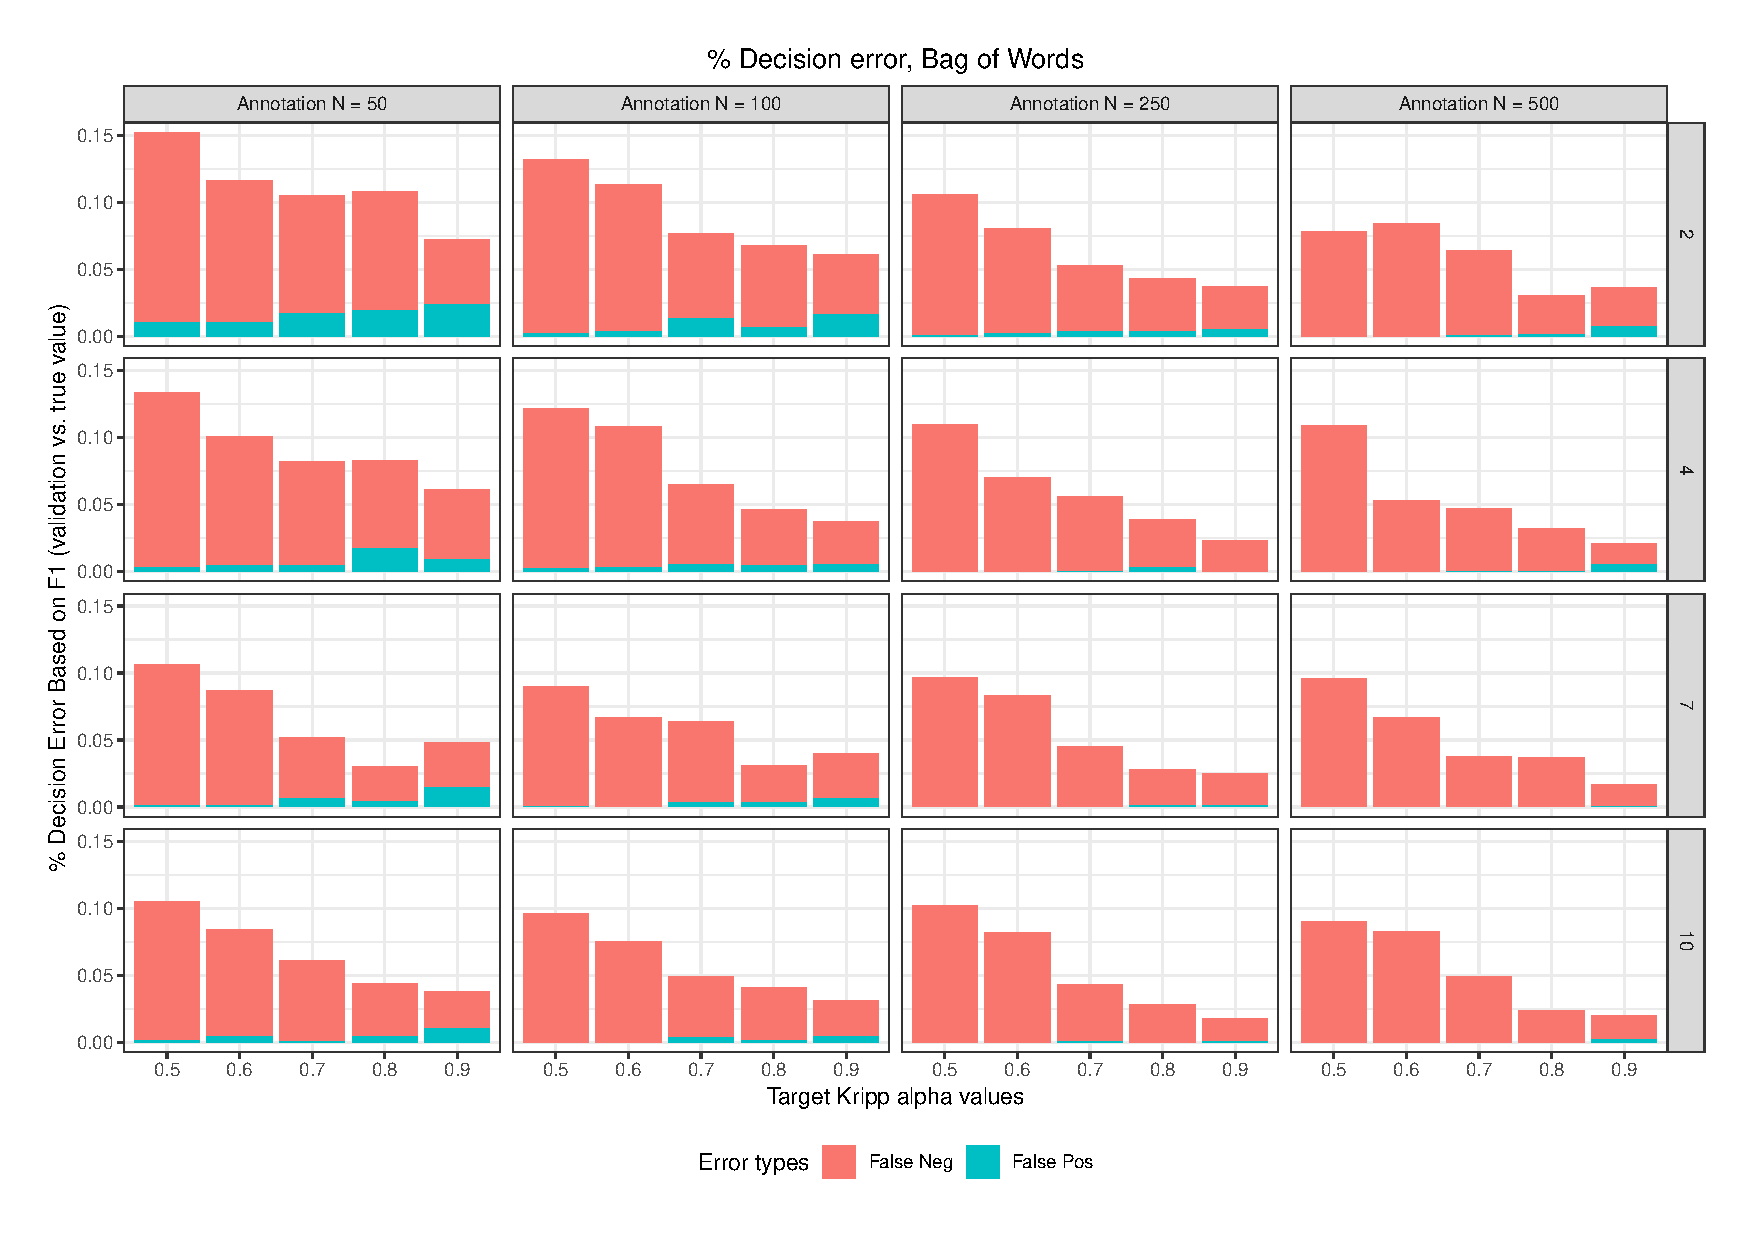
\includegraphics[clip, width=\linewidth, page = 1]{Results/BoW_summary_05.pdf} 
    \end{subfigure}
    \begin{subfigure}[t]{0.95\textwidth}
        \centering
        \includegraphics[clip, width=\linewidth, page = 2]{Results/BoW_summary_05.pdf} 
    \end{subfigure}
    
    \captionsetup{format=hang}
    \caption{Percentage of decision error and relative bias in F1 scores (over 1000 Simulations per each scenario), Bag-of-words.} 
    \label{fig:Figure4}
    \captionsetup{font=small}
    \caption*{Note: Upper panel = Proportion of cases (each simulation run) incorrectly conclude on classification performances. Lower panel = Relative bias in F1 scores among misclassified studies.}
\end{figure}     

As can be seen in Figure \ref{fig:Figure2}, it appears that using more \enquote{high-quality} materials for post-hoc validation have obvious and discernible consequences in the evaluation of classification quality of the automated procedures. Among 1000 replication of each scenarios, all of our experimental factors appears to decrease the decision error when using observed level of F1 scores to approximate the true (unknown) F1 score. The leftmost upper panel (2 coders, with 50 independent annotations per each coder) shows that in worst-case scenarios, using only two coders with handful of materials, coupled with sub-optimal reliability (K alpha of 0.5) produces approximately 30\% of study cases that incorrectly estimate the true F1 scores. Under the same combination of total number of coders and independent annotations per each coder, improving reliability at best marginally decreases the decision error (from 0.291 to 0.258). Yet as either total number of coders or independent annotations per each coder start to increase, we see that the total proportion of cases that incorrectly estimate the true F1 scores start to decrease substantially (the upper panel of Figure \ref{fig:Figure2}) while the relative bias the bottom panel of Figure \ref{fig:Figure2}) also start to converge to unbiased estimates (towards 1). While there is no apparent overall main effect of the higher reliability in manual validation materials in terms of reducing the total number of decision error, using higher reliability manual validation materials tend to \textit{reduce} the magnitude of relative bias (i.e., under- or overestimation of the true F1 scores based on observed F1 score),  especially when , reducing the            


\section{Conclusion and Discussion: TBA}

    
    The aims of the current paper were twofold; we first wanted to provide a systematic overview of how the matter of validation is approached by the field at large, and second --- we wanted to provide simulation-based evidence of how various decisions taken in the training and validation phases of a study that relies on machine learning applications can have widely different implications. To this end, we first presented the results of a meta study of relevant journal articles, as well as designed a set of Monte Carlo simulations.
    
    The results from the first study show that, while automated text analysis methods are widely used in throughout social sciences, there is still strikingly little consistency in how various stages of these approaches, and more specifically, the validation of these methods, are reported. Very often, studies do not report \textit{any} validation metrics when using machine learning applications, or, when the do, these metrics are generally not consistent. 
    
    
    Coupled with the results from our second study (simulation-based inference), we find these insights to be rather concerning, since it is now becomes evident that the decisions that taken by the researchers throughout the research design play a huge role in the quality of the results.
    
    The results of this analysis confirm that the field of automated text analysis is still in its infancy. A common agreement upon quality standards is still missing – among authors as well as reviewers or editors. Nevertheless, it is maturing just like the field of manual content analysis was ten years ago.
    
    
    
    
    
    Our contribution should be read as a call for a thorough and systematic application of validation procedures in any publication drawing on automated text analysis procedures. At the same time, the study serves to benchmark the combination of reliability in gold standard/ ground truth and validity scores and warns against improper use of both to demonstrate the validity of the approach.
    
    -	Summary of what this paper did and what we found out:
	This study set out to assess the employment of validation measures in existing automated content analyses as well as the consequences of different levels of reliability in the Gold Standard for the results of such analyses. 
	
	To that end, we first presented the results of a meta study of relevant journal articles. The results of this analysis confirm that the field of automated text analysis is still in its infancies. A common agreement upon quality standards is still missing – among authors as well as reviewers or editors. Nevertheless, it is maturing just like the field of manual content analysis was ten years ago.  
	
	Moreover, we ran a set of Monte Carlo simulations for the two most popular approaches (supervised machine learning and dictionary approach) to explore the consequences of different degrees of reliability in the gold standard. The results show that using imperfect human judgments trickles down to the validity of the automated approaches in the sense that it indeed has systematic consequences for the evaluation of the proposed automated procedures. 
	
-	Reflect on our methodological approach (limitations)? 

-	Best practice / how to do automated analysis properly? 

-	Discussion/Implications: 
	Our contribution should be read as a call for a thorough and systematic application of validation procedures in any publication drawing on automated text analysis procedures.
	
	Responsibility of science in a post-truth era --  Transparency, apply traceable procedures to open the black box of automated text analyses 
	
	Computers are not inherently correct -- validity checks are crucial
	
	automated analysis takes time and resources, not just a cheap alternative to expensive manual coding 
	
    At the same time, the study serves to benchmark the combination of reliability in gold standard/ground truth and validity scores and warns against improper use of both to demonstrate the validity of the approach
    
	Relate back to the title: it shouldn't be garbage at all…? So how to avoid garbage instead of assessing the degree of stink? 


    
\printbibliography
%\newpage
%\begingroup
%\parindent 0pt
%\parskip 1ex
%\def\enotesize{\normalsize}
%\theendnotes
%\endgroup
\end{document}
